\contourlength{1.0pt}
\tikzset{>=latex} % for LaTeX arrow head

\colorlet{xcol}{blue!60!black}
\colorlet{myred}{red!80!black}
\colorlet{myblue}{blue!80!black}
\colorlet{mygreen}{green!40!black}
\colorlet{myorange}{orange!90!black}
\colorlet{mypurple}{red!50!blue!90!black!80}
\colorlet{mydarkred}{myred!80!black}
\colorlet{mydarkblue}{myblue!80!black}
\tikzstyle{xline}=[xcol,thick]
\tikzstyle{width}=[{Latex[length=5,width=3]}-{Latex[length=5,width=3]},thick]
\tikzset{
  traj/.style 2 args={xline,postaction={decorate},decoration={markings,
    mark=at position #1 with {\arrow{<}},
    mark=at position #2 with {\arrow{<}}}
  }
}
\def\tick#1#2{\draw[thick] (#1)++(#2:0.12) --++ (#2-180:0.24)}
\def\N{100} % number of samples

% CIRCLE on axis




% ENERGY vs. t - damped


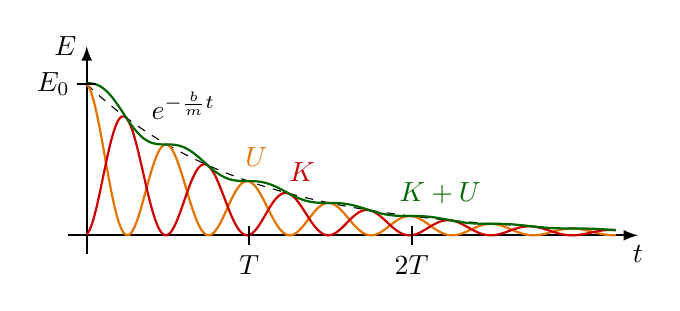
\begin{tikzpicture}
  \def\xmax{7.0} % max x axis
  \def\ymax{2.4} % max y axis
  \def\A{0.8*\ymax} % maximum extension
  \def\T{4.0}    % decay constant tau
  %\def\om{(2.5*360/(0.94*\xmax))} % angular frequency in degrees
  \def\om{(3.2*2*pi/(0.94*\xmax))} % angular frequency in radians
  \def\W{(sqrt((\om)^2-1/\T/\T))} % omega underdamped
  
  % AXIS
  \draw[->,thick] (0,-0.1*\ymax) -- (0,\ymax) node[left] {$E$};
  \draw[->,thick] (-0.1*\ymax,0) -- (\xmax,0) node[below] {$t$};
  
  % PLOT
  \draw[dashed,samples=\N,smooth,variable=\x,domain=0:0.96*\xmax]
    plot(\x,{\A*exp(-2*\x/\T)});
  \draw[xline,myorange,samples=100+\N,smooth,variable=\x,domain=0:0.96*\xmax]
    plot(\x,{\A*exp(-2*\x/\T)*cos(180/pi*\W*\x)^2});
  \draw[xline,myred,samples=100+\N,smooth,variable=\x,domain=0:0.96*\xmax]
    %plot(\x,{\A*exp(-\x/\T)*sin(180/pi*\W*\x)^2});
    plot(\x,{\A*exp(-2*\x/\T)*( 1/\T/\om*cos(180/pi*\W*\x) + \W/\om*sin(180/pi*\W*\x) )^2});
  \draw[xline,mygreen,samples=100+\N,smooth,variable=\x,domain=0:0.96*\xmax]
    plot(\x,{\A*exp(-2*\x/\T)*(cos(180/pi*\W*\x)^2 + ( 1/\T/\om*cos(180/pi*\W*\x) + \W/\om*sin(180/pi*\W*\x) )^2 )});
  \node[above right=0] at (0.1*\xmax,{\A*exp(-2*0.1*\xmax/\T)}) {$e^{-\frac{b}{m}t}$};
  \node[above right=0,myorange] at (0.27*\xmax,{\A*exp(-2*0.27*\xmax/\T)}) {$U$};
  \node[above right=0,myred] at (0.35*\xmax,{\A*exp(-2*0.35*\xmax/\T)}) {$K$};
  \node[above right=0,mygreen] at (0.55*\xmax,{\A*exp(-2*0.55*\xmax/\T)}) {$K+U$};
  \tick{0,\A}{0} node[left=-1,scale=1] {$E_0$};
  \tick{{2*pi/\W},0}{90} node[below,scale=1] {$T$};
  \tick{{4*pi/\W},0}{90} node[below,scale=1] {$2T$};
  
\end{tikzpicture}
